\documentclass{article}
\usepackage[utf8]{inputenc}
\usepackage{pgfplots}
\pgfplotsset{width=10cm,compat=1.9}
\usepackage{amsmath,amssymb,amsthm}
\usepackage{graphicx}
\usepackage{float}
\usepackage{blindtext}
\usepackage{hyperref}
\usepackage{verbatim}
\hypersetup{
    colorlinks=true,
    linkcolor=blue,
    filecolor=magenta,      
    urlcolor=cyan,
    pdftitle={Overleaf Example},
    pdfpagemode=FullScreen,
    }
\usepackage[slovene]{babel}

\newcounter{example}[section]
\newenvironment{example}[1][]{\refstepcounter{example}\par\medskip
   \noindent \textbf{Naloga~\theexample. #1} \rmfamily}{\medskip}

\newtheorem*{zgled}{Zgled}

\title{Eksponentna funkcija}
\author{Bor Bregant}
\date{\vspace{-5ex}}

\begin{document}

\maketitle

\section{Funkcija $f(x)=a^x$, kjer je $a>0$ in $a=1$.}
Primeri:
\begin{itemize}
    \item $f(x)=2^x$
    \item $x \mapsto 4^x$
    \item $f(x)=\left(\frac{\sqrt{3}}{10}\right)^x$
\end{itemize}

\subsection{Družina funkcija $f(x)=a^x; a>1$}
Oglejmo si primer $a=2$, torej $f(x)=2^x$. Tabelirajmo vrednosti in narišimo graf.

\begin{minipage}[c]{0.3\textwidth}
\vspace{0pt}
\begin{tabular}{|c|c|}
\hline
$x$  & $y=2^x$       \\ \hline
$-2$ & $\frac{1}{4}$ \\
$-1$ & $\frac{1}{2}$ \\
0    & 1             \\
1    & 2             \\
2    & 4             \\ \hline
\end{tabular}
\vspace{0pt}
\end{minipage}
\noindent
\begin{minipage}[c]{0.3\textwidth}
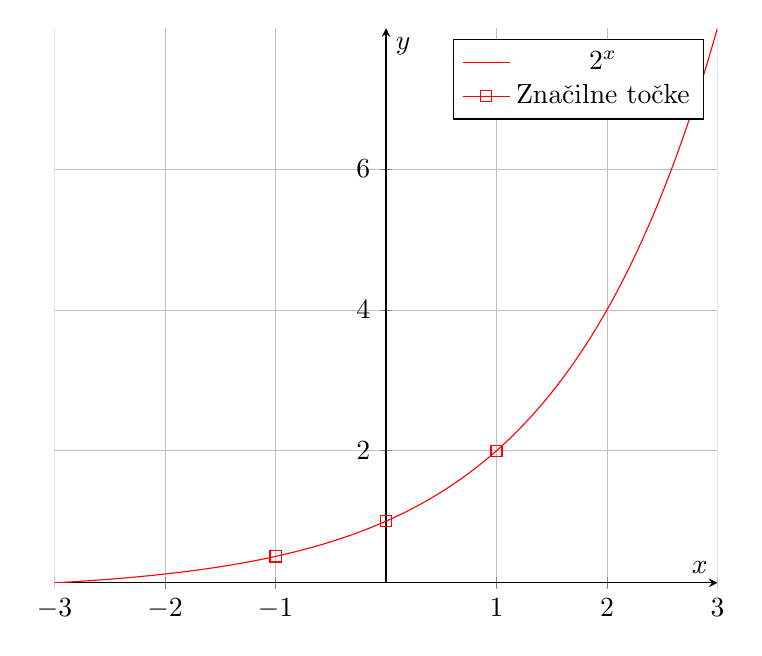
\begin{tikzpicture}
\begin{axis}[
    xlabel = \(x\),
    ylabel = {\(y\)},
    axis lines=middle,
    grid=both, grid style={line width=.1pt, draw=gray!10},
    major grid style={line width=.2pt,draw=gray!50},
]
\addplot [domain=-3:3, samples=100, color=red]
{2^x};
\addlegendentry{\(2^x\)}
\addplot[color=red, mark=square] coordinates {(-1,0.5)};
\addplot[color=red, mark=square] coordinates {(1,2)};
\addplot[color=red, mark=square] coordinates {(0,1)};\addlegendentry{Značilne točke}
\end{axis}
\end{tikzpicture}
\end{minipage}

\textbf{Lastnosti funkcij $f(x)=a^x; a>1$}
\begin{itemize}
    \item $D_f=\mathbb{R}$
    \item $Z_f=(0,\infty)$
    \item začetna vrednost $f(0)=1$
    \item značilne točke $(0,1),(1,a),\left(-1,\frac{1}{a}\right)$
    \item naraščajoča
    \item navzdol omejene z $0$, navzgor neomejene
    \item graf se proti $-\infty$ asimptotsko približuje abscisni osi
    \item so bijektivne
    \item so konveksne.
\end{itemize}

Pomembna je tudi funkcija $e^x$, kjer je $e=1+\frac{1}{1}+\frac{1}{1\cdot 2}+\frac{1}{1\cdot 2\cdot 3}+\cdots\approx2,72$ iracionalno \textit{eulerjevo} število.

\subsection{Družina funkcija $f(x)=a^x; 0<a<1$}

Oglejmo si $f(x)=\left(\frac{1}{2}\right)^x$. Ker je $\left(\frac{1}{2}\right)^x=2^{-x}$, lahko ta graf dobimo z zrcaljenjem grafa $y=2^x$ čez ordinatno osjo.

\begin{minipage}[c]{0.3\textwidth}
\vspace{0pt}
\begin{tabular}{|c|c|}
\hline
$x$  & $y=\left(\frac{1}{2}\right)^x$       \\ \hline
$-1$ & $2$ \\
0    & 1             \\
1    & $\frac{1}{2}$             \\ \hline
\end{tabular}
\vspace{0pt}
\end{minipage}
\noindent
\begin{minipage}[c]{0.3\textwidth}
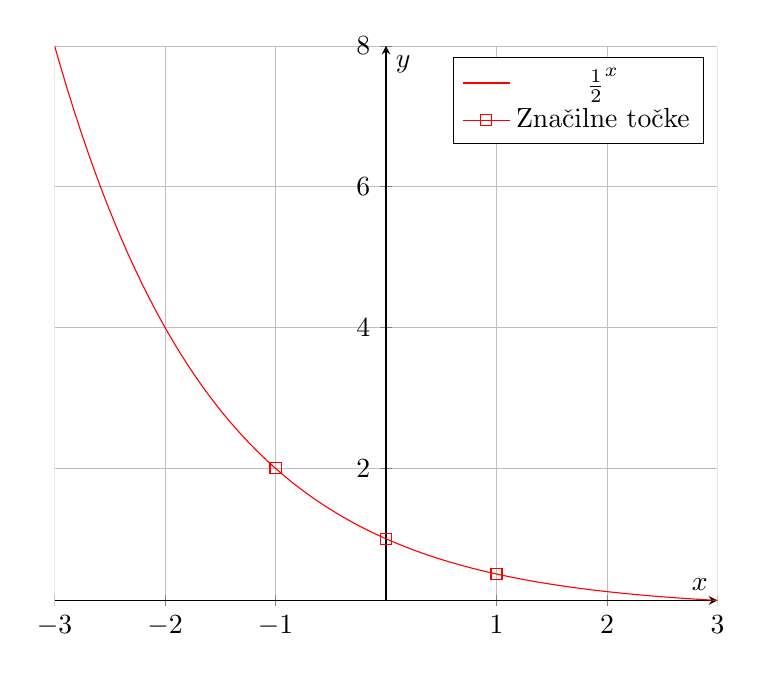
\begin{tikzpicture}
\begin{axis}[
    xlabel = \(x\),
    ylabel = {\(y\)},
    axis lines=middle,
    grid=both, grid style={line width=.1pt, draw=gray!10},
    major grid style={line width=.2pt,draw=gray!50},
]
\addplot [domain=-3:3, samples=100, color=red]
{0.5^x};
\addlegendentry{\(\frac{1}{2}^x\)}
\addplot[color=red, mark=square] coordinates {(1,0.5)};
\addplot[color=red, mark=square] coordinates {(-1,2)};
\addplot[color=red, mark=square] coordinates {(0,1)};\addlegendentry{Značilne točke}
\end{axis}
\end{tikzpicture}
\end{minipage}

\textbf{Lastnosti funkcij $f(x)=a^x; a>1$}
\begin{itemize}
    \item $D_f=\mathbb{R}$
    \item $Z_f=(0,\infty)$
    \item začetna vrednost $f(0)=1$
    \item značilne točke $(0,1),(-1,a),\left(1,\frac{1}{a}\right)$
    \item padajoča
    \item navzdol omejene z $0$, navzgor neomejene
    \item graf se proti $\infty$ asimptotsko približuje abscisni osi
    \item so bijektivne
    \item so konveksne.
\end{itemize}

\begin{zgled}
    \begin{itemize}
    \item Določimo eksponentno funkcijo $f(x)=a^x$, katere graf poteka skozi $A(2,9)$. Nato v isti koordnatni sistem narišimo $f(x), f(x+1), f(x+1)-1, f(-x), |f(x)-3|$.
    \end{itemize}
\end{zgled}

\begin{example}
V isti koordinatni sistem nariši grafe funkcij\\
(a) $f(x)=3^x, g(x)=3^x-2, h:x\mapsto 3^{x-2}$\qquad (b) $f(x)=2^{-x}, g(x)=\frac{3}{2}2^{-x}$
\end{example}
\begin{example}
Zapiši tri čim lepše točke grafa $f(x)=2^{x-2}-1$. Nato nariši grafe $f(x)$, $g(x)=|f(x)|$ in $h(x)=f(|x|)$.. Zapiši še ničle, z.v., $D_f$, $Z_f$ in enačbo asimptote.
\end{example}

\begin{example}
    Nariši $f(x)=-3\cdot 2^{x-1}$ in $g(x)=\frac{1}{3^x}-1$.
\end{example}

\begin{example}
Za funkcijo $f(x)=-2^x+2$ zapiši začetno vrednost, ničle, enačbo vodoravne asimptote in nariši njen graf. Poišči še predpis funkcije $g$, ki je dobljena tako, da graf $f$ premaknemo za vektor $(1,-1)$.
\end{example}


\subsection{Eksponentna enačba}

Tri skupine eksponentnih enačb in postopek reševanja:\\
\begin{tabular}{|l|l|l|}
\hline
Vrsta enačbe           & Postopek reševanja &Primer                      \\ \hline
$a^{f(x)}=a^{g(x)}$             & $f(x)=g(x)$  &$3^{x-1}=3^{2x+2}$                            \\
$a^{f(x)}=b^{f(x)}$             & $f(x)=0$    &$5^{2x}=(\frac{1}{2})^{2x}$                          \\
Nova spremenljivka (opazimo $\square^{2x} + \square^x+\square$ ali pa $\square^{-x}$)             & $t=\square^x$    &$\cdots$        \\
$\textcolor{red}{a^{f(x)}=b}$ & \textit{Logaritmiranje}&$2^{x-3}=5$\\\hline
\end{tabular}

\begin{zgled}
    Rešimo enačbo $9^{x-3}=3\sqrt{3}$. (naloga z mature)
\end{zgled}
\begin{zgled}
    Rešimo enačbo $4\cdot 2^{2x+1}=\frac{1}{8}$.
\end{zgled}
\begin{zgled}
    Rešimo enačbo $2\cdot 4^{x+3}=32^{x-1}$.
\end{zgled}
\begin{zgled}
    Rešimo enačbo $9\cdot 3^{2x-2}=\sqrt[9]{27^{x+1}}$.
\end{zgled}
\begin{zgled}
    Poišči presečišča za $f(x)=4^{x-1}$ in $g(x)=8^{2x-3}$.
\end{zgled}
\begin{zgled}
    Rešimo enačbo $4\cdot 2^{2x+1}=\frac{1}{8}$.
\end{zgled}
\begin{zgled}
    Rešimo enačbo $5^{x+1}+5^{x+2}=6$.
\end{zgled}
\begin{zgled}
    Rešimo enačbo $2^{x-3}+3\cdot 2^{x-1}-2^x=20$.
\end{zgled}

\begin{zgled}
    Rešimo enačbo $2\cdot 7^x-11=21\cdot 7^{-x}$.
\end{zgled}
\begin{zgled}
    Rešimo neenačbo $3^{x-1}>3$.
\end{zgled}

\begin{example}
    Reši enačbe:\\
    (a) $5^x=125$\qquad (b) $4^{x-1}=16$ \qquad (c) $2^{x-3}=4^3$ \qquad (d) $5^{x-1}=\frac{1}{25}$ \\\qquad (e) $\left(\frac{8}{27}\right)^x=\frac{3}{2}$ \qquad (f) $4^x=-8$ \qquad (g) $\sqrt{27}=9^{1-x}$ \qquad (h) $5^{3x}=5^{7x-2}$ \qquad \\ (i) $4^{t^2}=4^{6-t}$
\end{example}
\begin{example}
    Reši enačbe:\\
    (a) $5^x=7^x$ \qquad (b) $4^{x-4}=6^{4-x}$ \qquad (c) $2^{x^2-x-6}=1$
\end{example}
\begin{example}
    Reši enačbe:\\
    (a) $3^{x+2}+3^x=90$ \qquad (b) $2^{2x-1}+3\cdot 2^{2x}-2^{2x+2}+1=0$ \qquad (c) $3^{2x}+3^x=12$ \qquad (d) $4^x+1=17\cdot 2^{x-2}$
\end{example}
\begin{example}
    Reši neenačbe (pomagaj si z grafom):\\
    (a) $3^{x+2}-1>0$ \qquad (b) $5^{x+1}\leq \frac{1}{5}$ \qquad (c) $2^x>1-x$.
\end{example}
\begin{example}
    V isti koordinatni sistem nariši grafa funkcij $f(x)=e^{-x-2}$ in $g(x)=e^x$ in izračunaj njuno presečišče.
\end{example}

\section{Logaritem}

Defincija: $\log_a x=y \iff a^y=x$, kjer $x>0,a>0,a\neq 1$. Število $a$ imenujemo \textit{osnova logaritma}, $x$ pa \textit{logaritmand}.\\
Posebej označimo $\log x=\log_{10} x$ (desetiški logaritem) in $\ln x=\log_e x$ (naravni logaritem).
\begin{zgled}
    \begin{itemize}
    \item $\log_2 16=4$, saj je $2^4=16$
    \item $\log_2 \frac{1}{4}=-2$, saj je $2^{-2}=\frac{1}{4}$
    \item $\log_{\frac{1}{5}}1=0$
    \item $\log_5 (-10)$ ne obstaja, saj je logaritmand negativen
    \item $\ln e=1$
    \end{itemize}
\end{zgled}
\begin{zgled}
    Izrazimo in določimo $x$, če je $\log_8 x=-\frac{2}{3}$.\\
    Izrazimo in določimo $x$, če je $0.7^x=0.49$.
    
\end{zgled}

\textbf{Pravili:}
\[a^{\log_a x}=x \qquad \text{in} \qquad \log_a a^x=x\]

\begin{zgled}
    Izračunajmo $\log_3 3^{0.4}$ in $4^{\log_4 8}$\\
    
\end{zgled}

\begin{example}
    Izračunaj brez kalukatorja in nato preveri s kalkulatorjem:\\
    (a) $\log_2 32$ \qquad (b) $\log_{\frac{1}{2}}16$ \qquad (c) $\log 0.001$.
\end{example}
\begin{example}
    Določi $x$, če je:\\
    (a) $2^x=16$ \qquad (b) $\log_x 16=4$ \qquad (c) $\log_x 64=3$
\end{example}
\begin{example}
    Izračunaj:\\
    (a) $2^{\log_2 4}$ \qquad (b) $7^{\log_7 0.6}$
\end{example}
\begin{example}
    Med katerima zaporednima celima številoma leži število:\\
    (a) $\log 49$ (brez kalukatorja) \qquad (b) $\ln (8.9\cdot 10^9)$ (pomagaj si s kalkulatorjem)
\end{example}
\begin{example}
    S kalkulatorjem izračunaj na dve decimalki natančno:\\
    (a) $2\log 6 - 13\ln 2 + \log_3 5$
\end{example}

\subsection{Pravila za računanje logaritmov}

\begin{itemize}
    \item $\log_a (x_1 \cdot x_2) =\log_a x_1 + \log_a x_2$
    \item $\log_a \frac{x_1}{x_2} =\log_a x_1 - \log_a x_2$
    \item $\log_a x^r = r\cdot\log_a x$
    \item $\log_b x=\frac{\log_a x}{\log_a b}$
\end{itemize}
\begin{comment}
\begin{zgled}
    Zapišimo $\log_a\left(a^4\frac{\sqrt{b}}{c^3}\right)$ z logaritmi z osnova $a$.\\
    Zapišimo $\log 2.88$ z logaritmi praštevil.\\
    Skrčimo izraz $\log_2 5 \cdot \log_5 \frac{1}{16}$.\\
    Z antilogaritmiranjem izrazi $y$ v enačbi $\log_2 y=\log_2 32 +\log_2 4x^2-\frac{1}{5}\log_2 1024$.
\end{zgled}
\begin{example}
    Izrazi z logaritmi z osnovo $a$:\\
    (a) $\log_a (bcd)$ \qquad (b) $\log_a \frac{a^2}{bd}$ \qquad (c) $\log_a \sqrt{b\sqrt{c}}$
\end{example}
\begin{example}
    Izrazi z logaritmi praštevil:\\
    (a) $\log 12$ \qquad (b) $\log\frac{345}{343}$ \qquad (c) $\log 250$
\end{example}
\begin{example}
    Izrazi $x$ (oziroma antilogaritmiraj):\\
    (a) $\log_a x=2\log_a 5 + 3\log_a 2$ \qquad (b) $2\log_a x= \frac{1}{3}\log_a 16-\frac{1}{3}\log_a 2$\\
    (c) $\log_a x=\frac{1}{2}\log_a(y+z)-\frac{1}{2}\log_a(y-z)$ \qquad \\(d) $\log x=\frac{1}{4}\log 2+\frac{1}{3}\log(u+v)-3\log u-2\log v$
\end{example}
\begin{example}
    Poenostavi oziroma izračunaj:\\
    (a) $2\log_a b+5\log_a c$ \qquad (b) $6+\log\frac{a}{10^6}$ \qquad (c) $\log x+\log x^4-2\log\frac{1}{x^2}$ \qquad (d) $(\ln x^2):(\ln x)$ \qquad (e) $\log 200-\log 21+\log 105$ \qquad (f) $\ln e^2-10^{\log\frac{1}{3}}-3\log_5 \sqrt{5}$
\end{example}
\begin{example}
    S prehodom na novo osnovo izračunaj oziroma poenostavi:\\
    (a) $\log_5 2 \cdot \log_2 5$ \qquad (b) $\log_{\frac{1}{2}}5\cdot \log_5 4$ \qquad (c) $\log_a b \cdot \log_b \sqrt{a}$
\end{example}
\end{comment}
\begin{zgled}
    Uporabi pravila logaritmov:\\
    $\log_5 x +  \log_5 \frac{1}{x}$\\
    $\log_a 10 - \log_a 2$\\
    $\log_2 (x+1)^2$\\
    $\log_3 x + 6\log_3 (x+1)$\\
    Z novo osnovo izračunaj $\log_5 2 \cdot \log_2 5$ in $\log_{\frac{1}{2}}5\cdot \log_5 4$.
\end{zgled}

\subsection{Logaritemska funkcija}

Loagritemska funkcija $f(x)=\log_a x (a>0)$ je inverzna funkcija eksponentni funkciji $f(x)=a^x$.
\begin{zgled}
    Poiščimo inverzno funkcijo funkciji $f(x)=3^{\frac{x}{2}-1}$.\\
    
\end{zgled}

\subsubsection{Družina funkcij $f(x)=\log_a x, a>1$}

\begin{figure}[H]
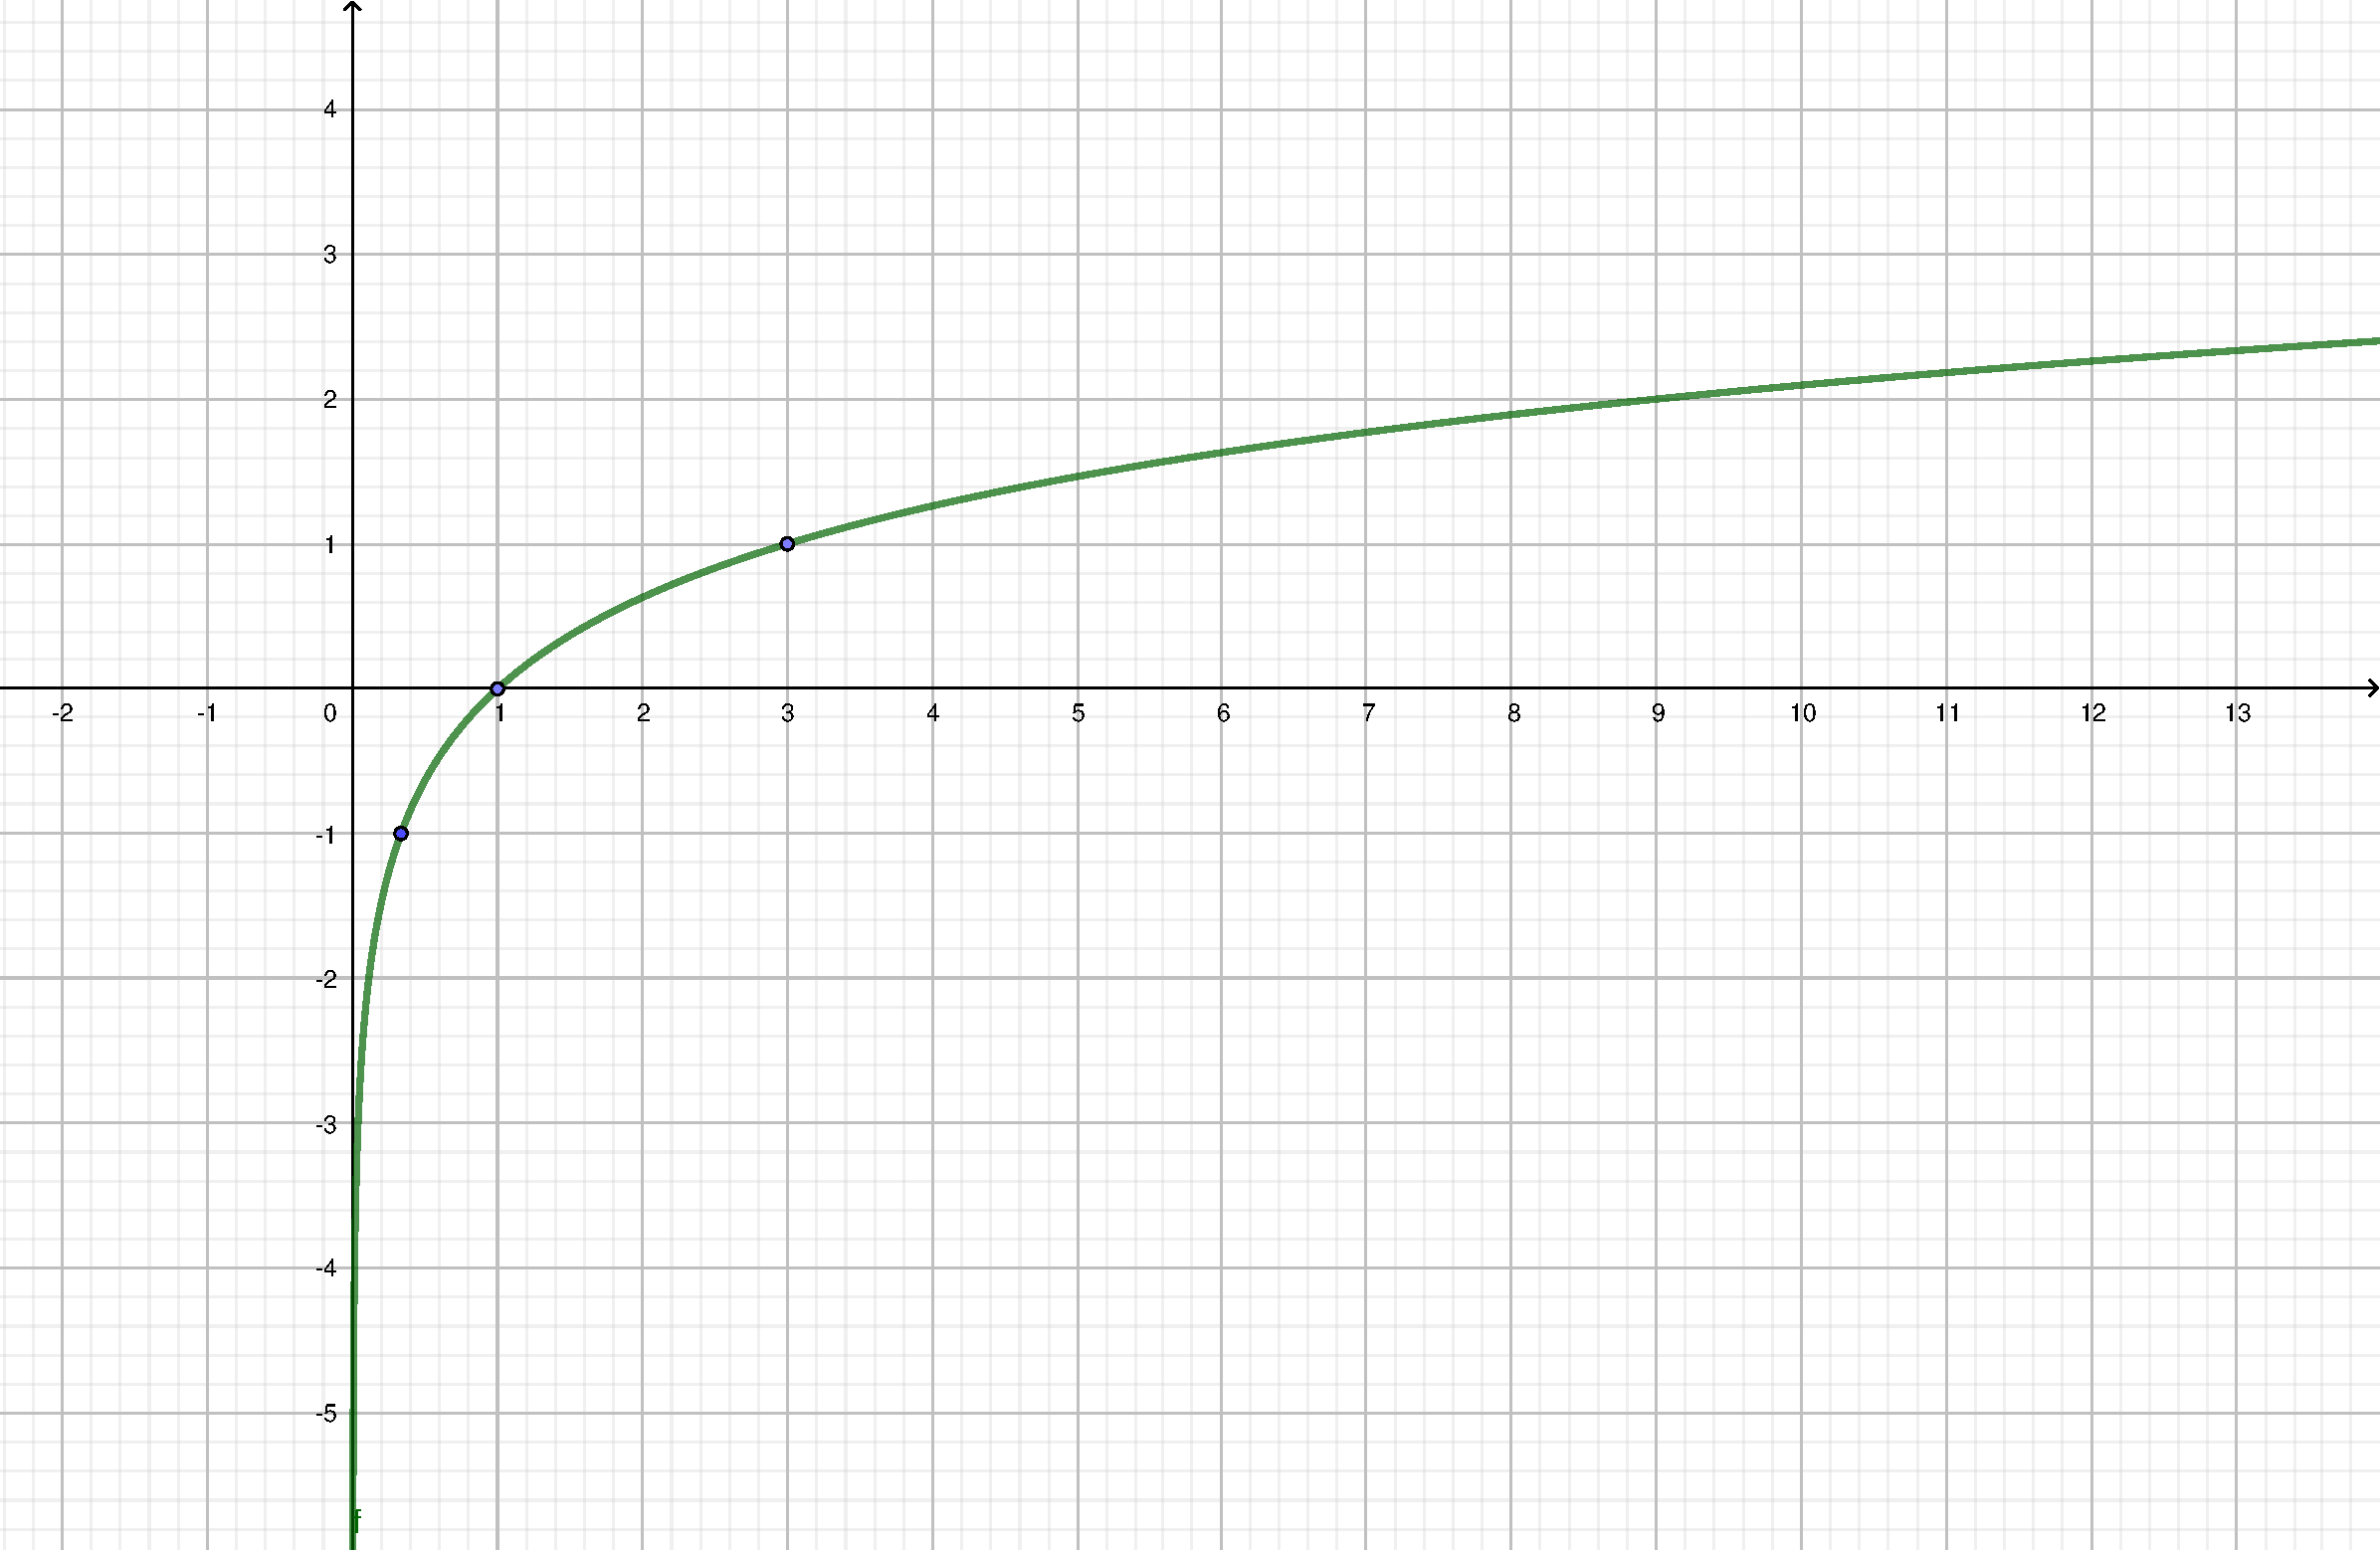
\includegraphics[width=0.7\textwidth]{logaritm.pdf}
\centering
\end{figure}

\textbf{Lastnosti funkcij $f(x)=\log_a x, a>1$}
\begin{itemize}
    \item $D_f= (0,\infty)$
    \item $Z_f=\mathbb{R}$
    \item ničla $x=1$
    \item značilne točke $(1,0), (a,1), (\frac{1}{a},-1)$
    \item naraščajoče
    \item navpična asimptota $x=0$
    \item neomejene navzgor in navzdol
    \item bijektivne
    \item konkavne
\end{itemize}

\begin{example}
    Ob grafu funkcije $f(x)=\log_{\frac{1}{2}}x$ napiši lastnosti družine funkcij $f(x)=\log_a x, 0<a<1$.\\
    \begin{figure}[H]
    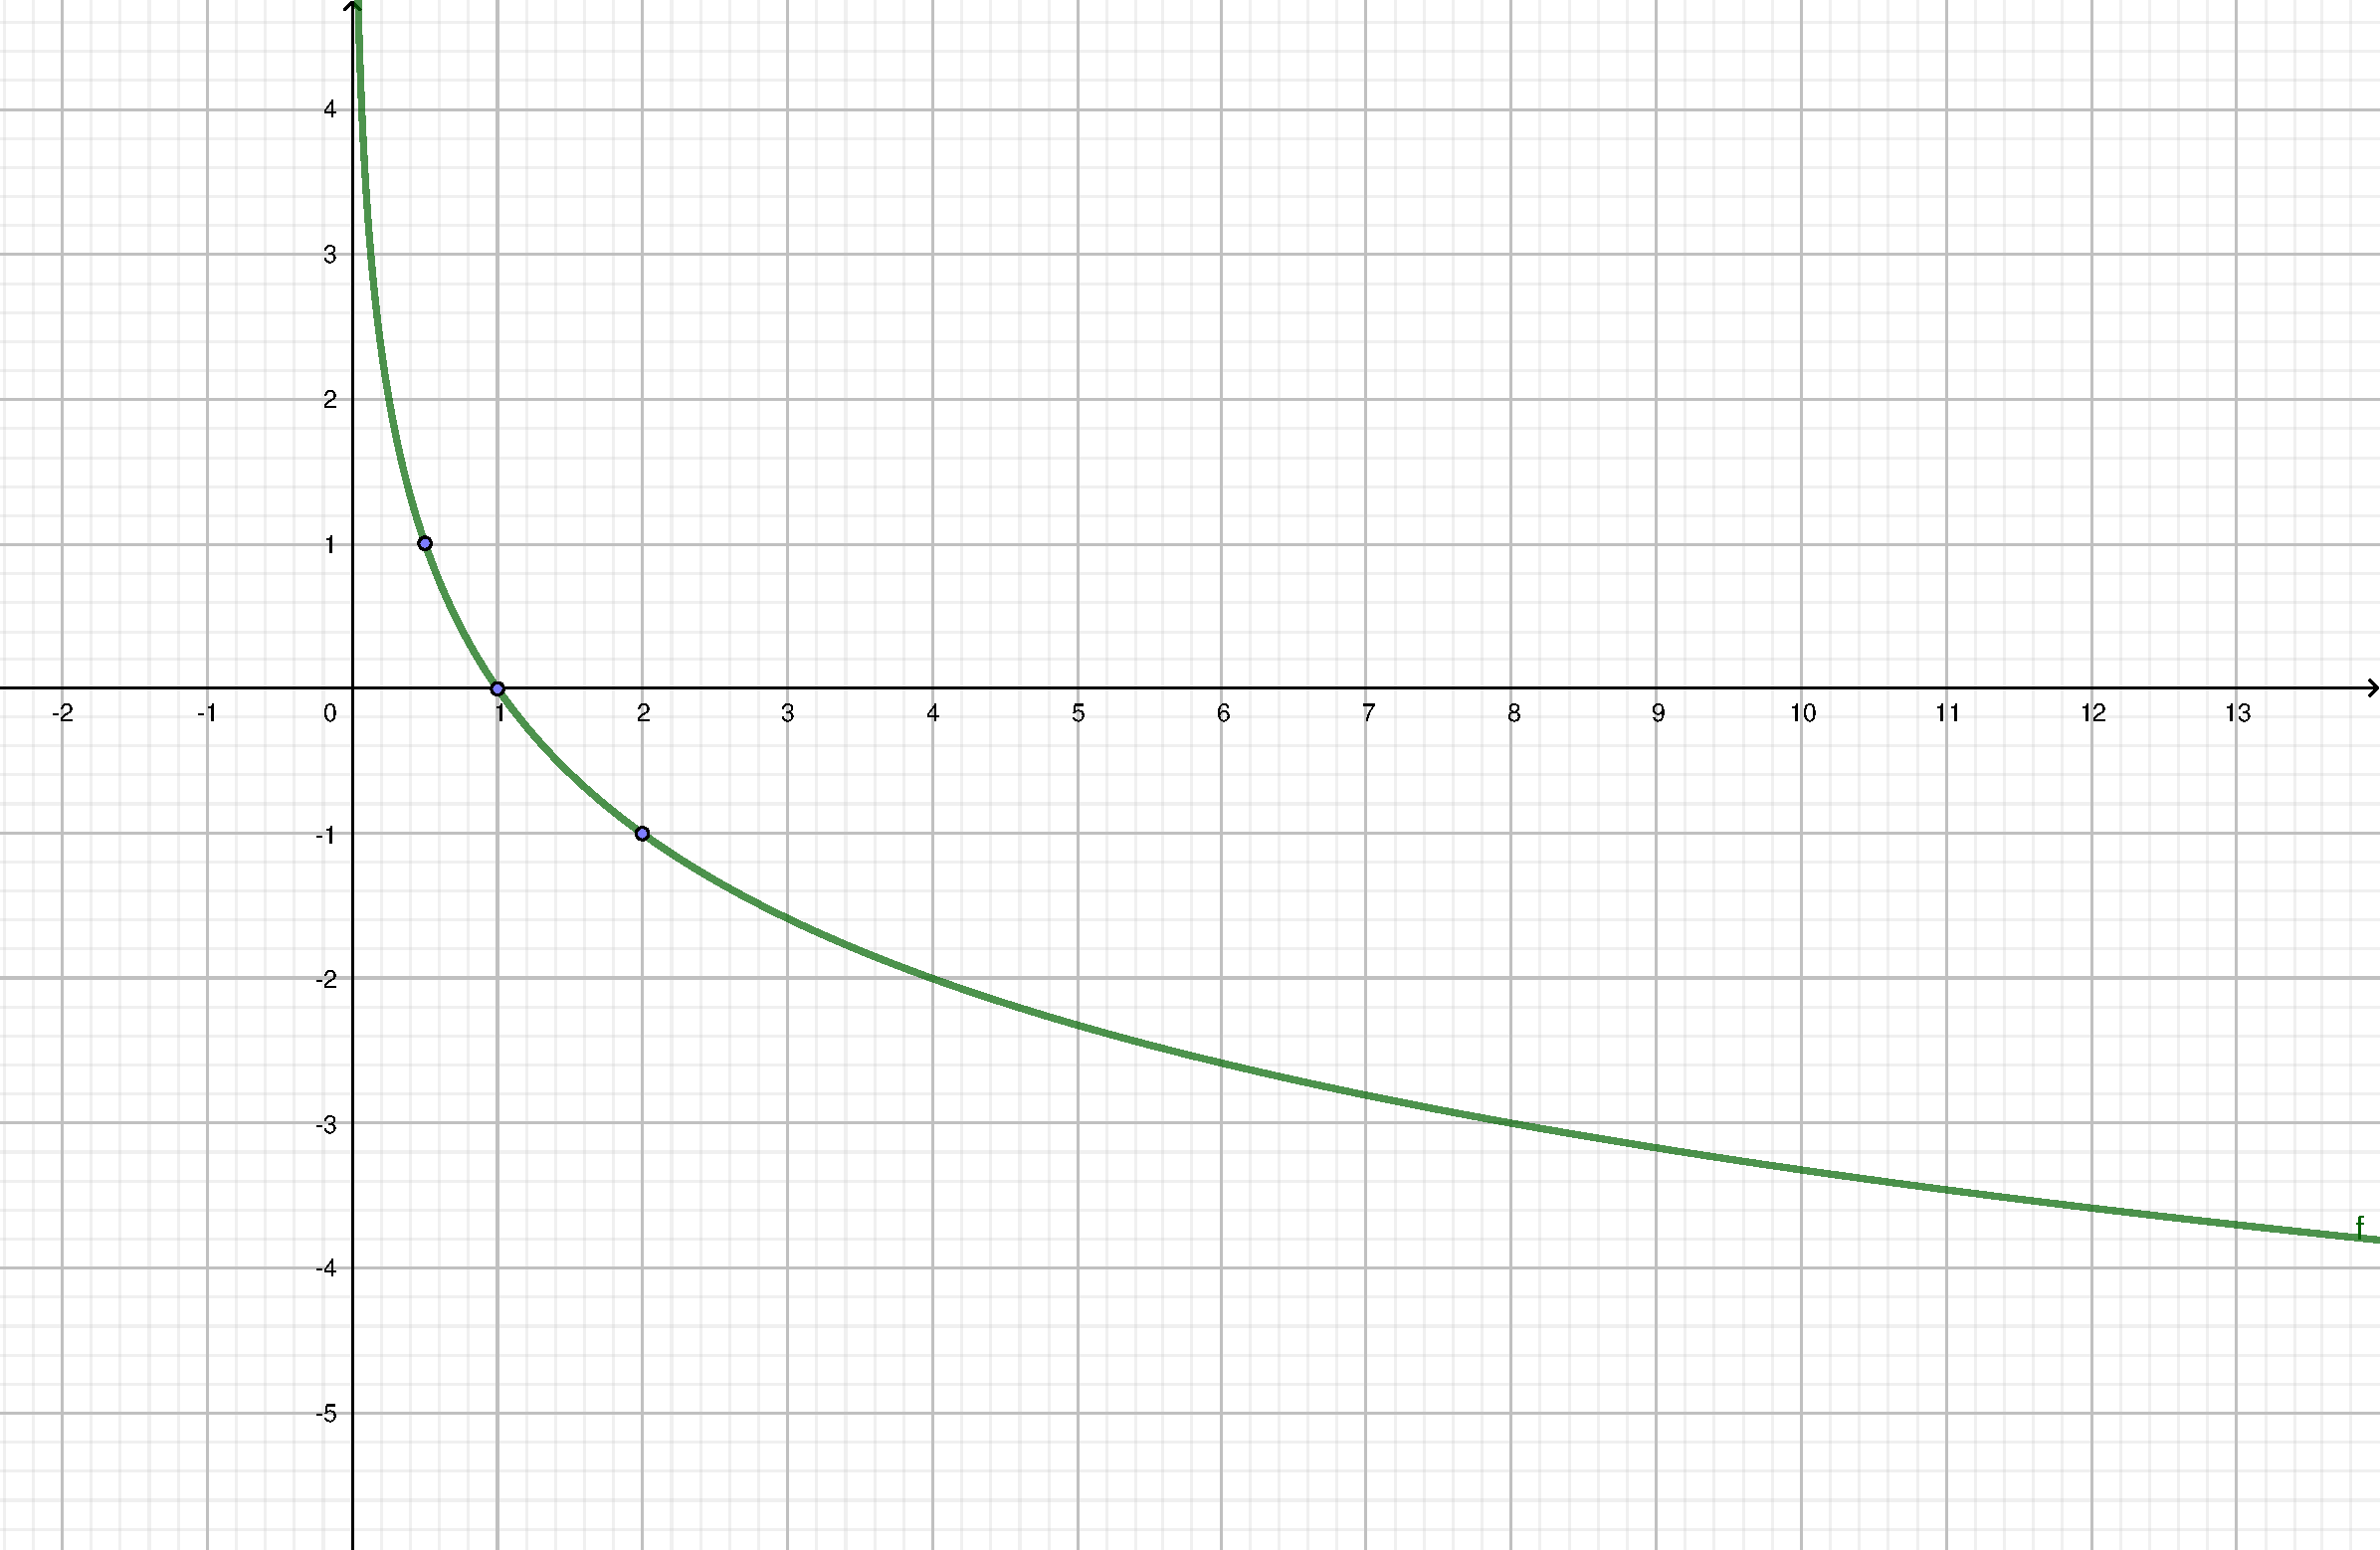
\includegraphics[width=0.7\textwidth]{logaritm1.pdf}
    \centering
    \end{figure}
\end{example}

\begin{zgled}
    Izračunajmo ničlo , narišimo graf in zapišimo definicijsko območje funkcije $f(x)=2\log_3 (x+3)$\\
\end{zgled}
\begin{example}
    Določi predpis funkcije $f(x)=\log_a x$, za katero velja $f(8)=3$. Nato tej funkciji poišči njen inverz. Funkcijo $f$ tudi nariši.
\end{example}

\subsection{Logaritemska enačba}

Pri teh enačbah je pomembno napraviti preizkus!

\begin{zgled}
    Rešimo naslednje enačbe:\\
    (a) $\log_{\frac{1}{5}}(3x-2)=-2$ (naloga z mature)\\
    (b) $\log(x-1)-\log x = \log(x+3)-\log(x-4)$\\
    (c) $\log_2(x+1)+\log_2 x=1$\\
    (d) $2\log^2 x-5\log x =3$\\
    (e) $x^{\log x}=10$\\
\end{zgled}
\begin{example}
    Kje graf funkcije $f(x)=1+\log_5 (x+2)$ seka premico $y=2$ in kje abscisno os.
\end{example}
\begin{example}
    Reši enačbe:\\
    (a) $\log(3x+1)=2$ \qquad (b) $\log_2 \sqrt{2x+1}=0.5$\\
    (c) $\log x+\log(x+1)=\log6$ \qquad (d) $\log_3(x+4)-\log_3 x=2$\\
    (e) $\ln(1-4x)-\ln x=1$ \qquad (f) $(\log x)(\log x+1)=2$\\
    (g) $\log_3 (1+\log_2(x+3))=1$ \qquad (h) $x^{1+\log x}=10^2$
\end{example}
\begin{example}
    Reši neenačbe:\\
    (a) $\log_3 x>0$ \qquad (b) $0<\log_2 (x+1)<3$
\end{example}
\begin{example}
    Reši enačbe:\\
    (a) $\log_3 x+\log_9 x=3$ \qquad (b) $2\log_7 x+\log_x 49=4$\\
    (c) $2^{\frac{x}{2}}=16$ \qquad (d) $2^x=3^{x+2}$
\end{example}


\begin{comment}
\section{Eksponentna in logaritemska funkcija v praksi}

\begin{zgled}
    Število bakterij se podvoji vsakih $15$ minut. Koliko bo bakterij po 8 urah, če je bila na začetku samo ena?\\
    Podvojitev implicira eksponentno rast, torej bo število bakterij po $t$ minutah enako $N(t)=N_0 \cdot 2^{\frac{t}{15}}$.\\
    Preostane nam le še izračun $N(8\cdot 60)=\ldots$
\end{zgled}
\begin{zgled}
    Bor položi na varčevalni račun banke 2000 evrov po obrestni meri $2\%$. Koliko časa mora varčevati, če želi imeti na računu 2015 evrov.
\end{zgled}
\begin{zgled}
    Razpadni čas
\end{zgled}
\end{comment}




\end{document}